\section{Skin}
The skin is a complex organ a ~\cite{elin2018}, it is interactive, self renewing and represents the first and primary defense line against hostile environment and it has several characteristics such as selective absoption, auto regeneration when injured, barrier to water loss, touch sensitivity ...etc ~\cite{joseph2020}. It represents the largest sensory organ (15\% of total body weight and a total area of 1.86 m²) ~\cite{sarah2021}, it has a highly adaptive structure that makes it vital for the survival of the human body, the balance between its static and dynamic properties makes it highly adaptive to the variations of the outer world ~\cite{eliana2022}.

\subsection{Skin Anatomy}
The skin is primary composed of 3 main layers as shown in the figure ~\ref{fig:skin}, each layer has its unique properties and functions ~\cite{sarah2021}.
\begin{description}
\item[Epidermis] the outer most layer which is constantly regenerating and it contains the pigment melanin that determins the skin color and it also represents a physical and biological barrier
\item[Dermis] the middle layer, it supports the flexibility and gives strength the epidermis and it is maily composed of connective tissue
\item[Hypodermis] the last layer which is composed of subcutaneous fat which gives it its properties of being a main support of the overall structure of the skin and shock absoption
\end{description}

%-----------figure skin structure/anatomy ----------------
\begin{figure}[htbp]
\begin{center}
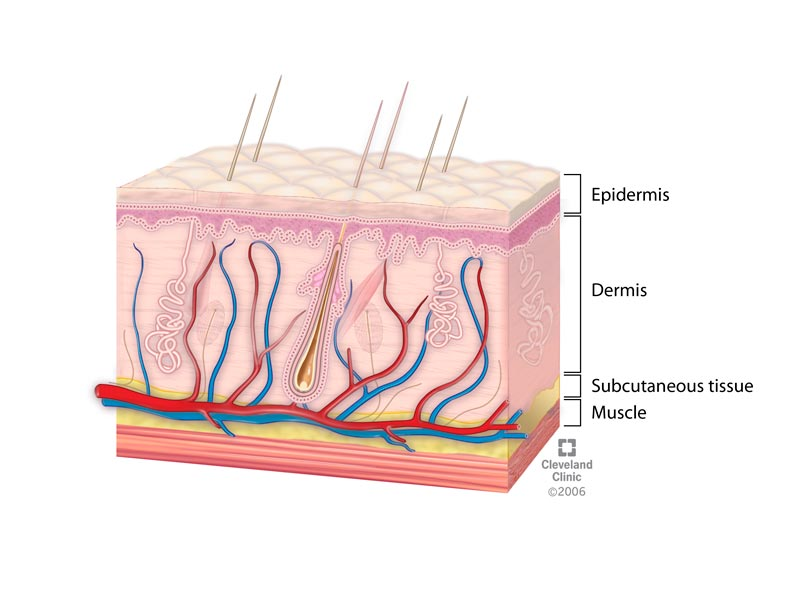
\includegraphics[width=15cm]{./chapter-01-general-medical-information/skin-anatomy.jpg}
\end{center}
\caption{Skin Anatomy ~\cite{fig-skin}}
\label{fig:skin}
\end{figure}

\subsection{Other entities also contained in the skin}
\begin{description}
\item[Hair]  provides protection agains minor trauma, thermoregulation and filtering functions such as nasal hair and eyelashes
\item[Sweat Glands] it is foucd across the entire body, it provides lubrication, temprerature regulation and salt and water balance.
\end{description}
there anatomies are shown in the figure ~\ref{fig:hair}

%-------------figure hair sweat glands-----------------------------
\begin{figure}[htbp]
\begin{center}
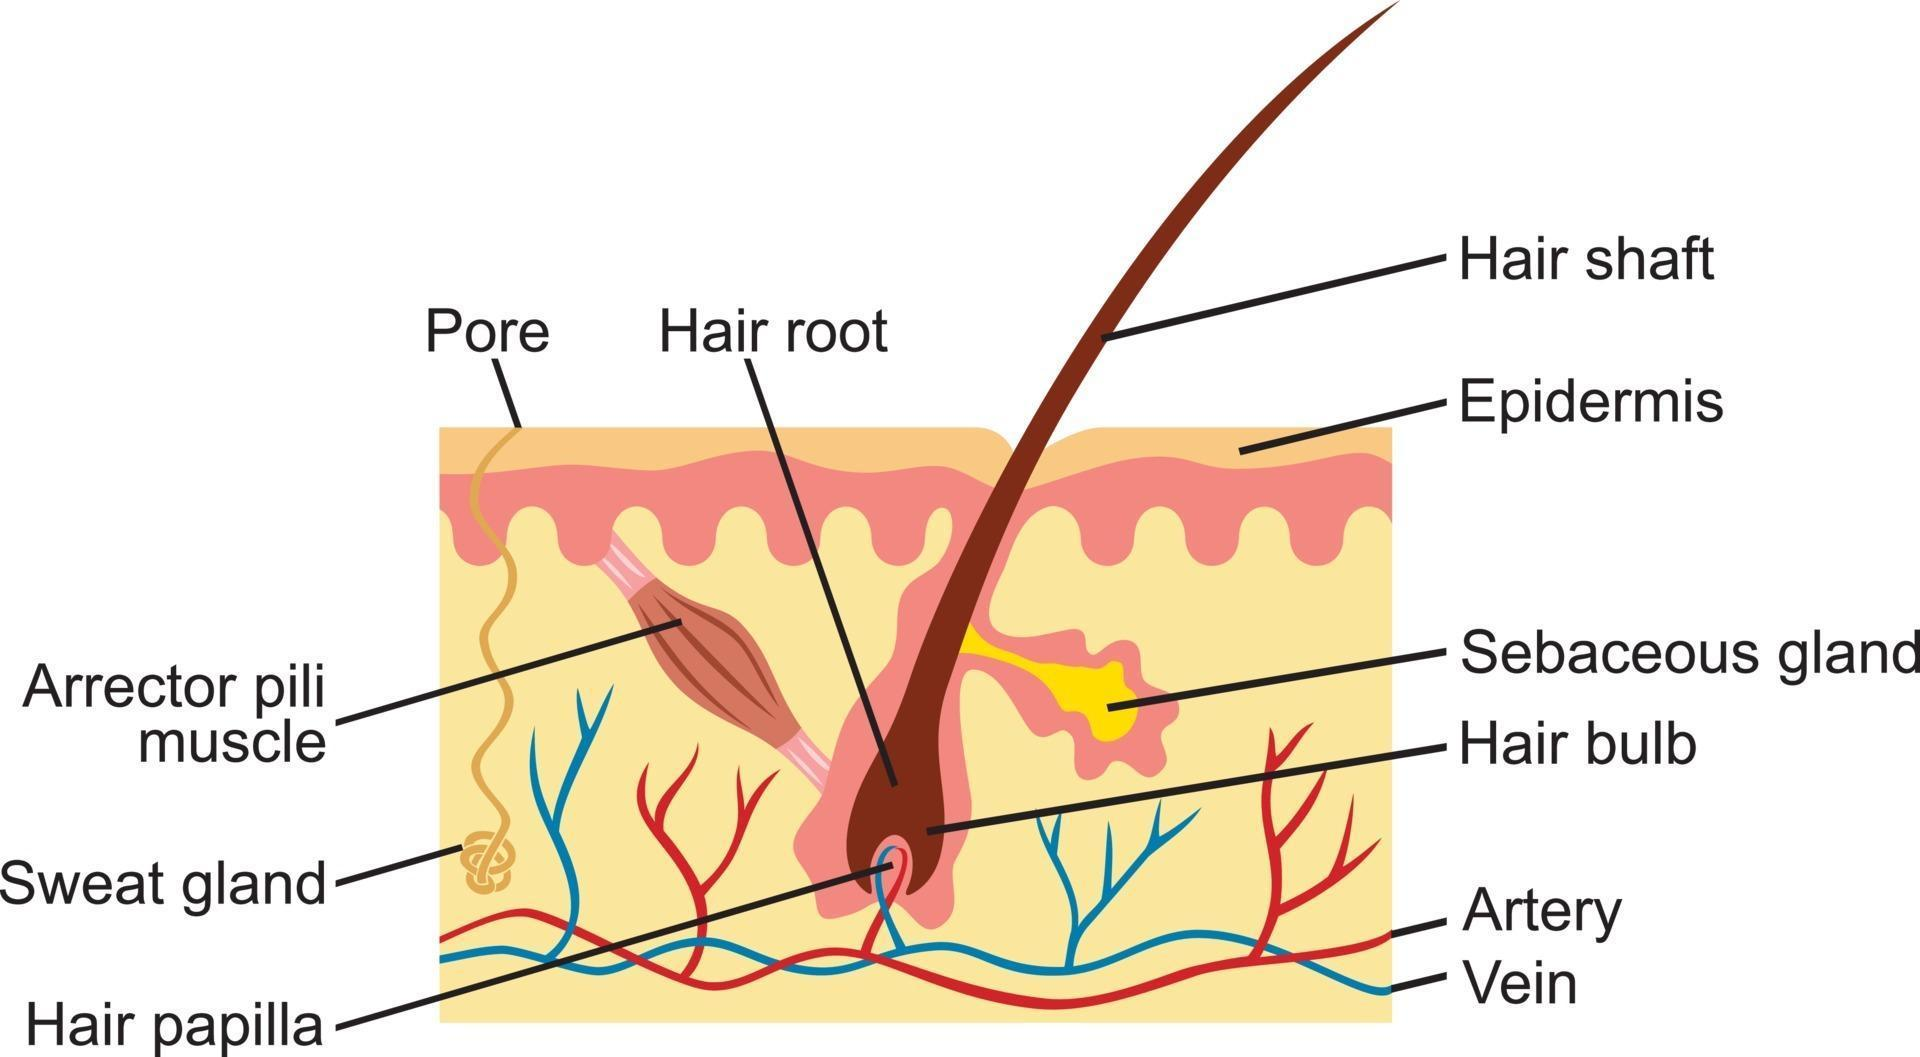
\includegraphics[width=15cm]{./chapter-01-general-medical-information/hair-sweat-gland.jpg}
\end{center}
\caption{Hair and Sweat Glands Anatomy ~\cite{fig-hair}}
\label{fig:hair}
\end{figure}


\subsection{Functions of the Skin}
The skin has 6 main functions that can be summarized as follows~\cite{sarah2021}
\begin{description}
\item[Protection]
            the skin is a direct interface between the entarnal organs and the environment so it works as a protective barrier against harmful objects and pathogens (innate/adaptive immunity and unltra-violet light protection  ~\cite{joseph2020}) as shown in figure ~\ref{fig:barrier}
            
\item[Thermostat]
            the skin works as a thermoregulator to keep the body at the optimal temperature of 37 C°, to achieve that is uses multiple strategies such as insensible perspiration, sweating ...etc
\item[Neural relay network]
            the skin contains a dense network of neural endings that works as receptors to various signals and provides sensations for touch, temperature and pain.
\item[Expression and communication]
            A more social function
            is the ability for skin to enable individuals to display
            emotions. It acts as an indicator of one’s physical state.
            Skin is an important component of the stress response as it
            acts as an immediate stress perceiver and as a target of
            stress responses.
            the skin also works as a social tool for interactions between human beings by indicatings the physical state of the individual and by showing sign of stress.
\item[Water storage]
            this skin works as a conservative barrier agains water and body fluids leakage (18-20\% of totla body water) as shown in figure ~\ref{fig:barrier}
\item[Synthesis of vitamin D]
            the skin reperesents the main site of vitamin D production when exposed to the sun, it exists in the plasma membranes of basal and suprabasal keratinocytes in its inactive form then it is converted to previtamin D3 then to Vitamin D in the liver and kidneys  ~\cite{joseph2020} as shown in figure ~\ref{fig:vitaminD}
\end{description}
        %----------figure skin protective barrier-------------
\begin{figure}[htbp]
\begin{center}
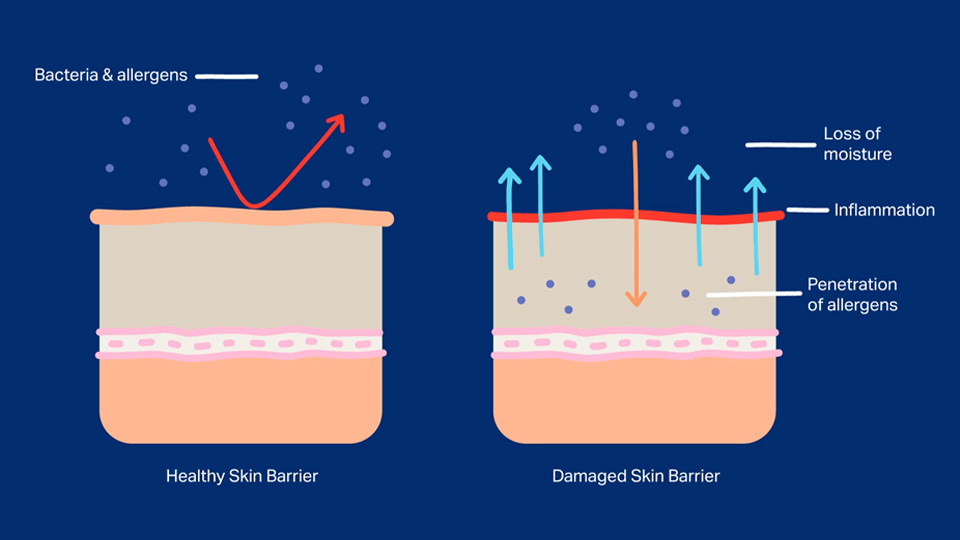
\includegraphics[width=15cm]{./chapter-01-general-medical-information/protective-barrier.jpg}
\end{center}
\caption{Protective/moisture Barrier Functions ~\cite{protectiveBarrier}}
\label{fig:barrier}
\end{figure}
        %-----------figure skin vitamin D-----------------
\begin{figure}[htbp]
\begin{center}
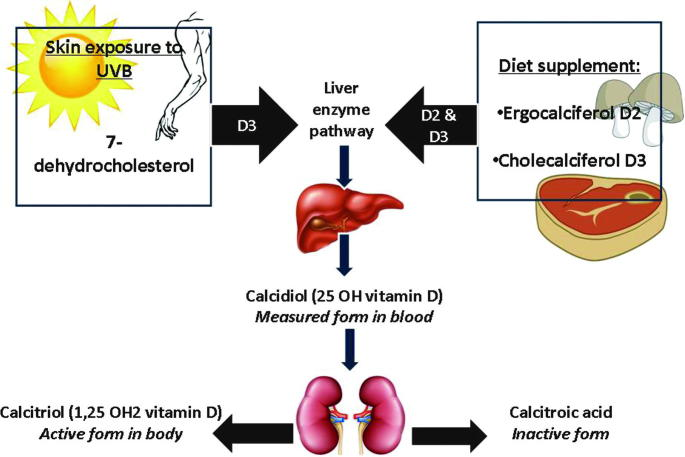
\includegraphics[width=10cm]{./chapter-01-general-medical-information/vitaminD.jpg}
\end{center}
\caption{Hair and Sweat Glands Anatomy ~\cite{vitaminD}}
\label{fig:vitaminD}
\end{figure}

